%% 
%% Copyright 2019-2024 Elsevier Ltd
%% 
%% This file is part of the 'CAS Bundle'.
%% --------------------------------------
%% 
%% It may be distributed under the conditions of the LaTeX Project Public
%% License, either version 1.3c of this license or (at your option) any
%% later version.  The latest version of this license is in
%%    http://www.latex-project.org/lppl.txt
%% and version 1.3c or later is part of all distributions of LaTeX
%% version 1999/12/01 or later.
%% 
%% The list of all files belonging to the 'CAS Bundle' is
%% given in the file `manifest.txt'.
%% 
%% Template article for cas-dc documentclass for 
%% double column output.

\documentclass[a4paper,fleqn]{cas-dc}

% If the frontmatter runs over more than one page
% use the longmktitle option.

%\documentclass[a4paper,fleqn,longmktitle]{cas-dc}

%\usepackage[numbers]{natbib}
%\usepackage[authoryear]{natbib}
\usepackage[authoryear,longnamesfirst]{natbib}
\usepackage{algorithm}
\usepackage{algpseudocode}
\usepackage{stfloats}

%%%Author macros
\def\tsc#1{\csdef{#1}{\textsc{\lowercase{#1}}\xspace}}
\tsc{WGM}
\tsc{QE}
%%%

% Uncomment and use as if needed
%\newtheorem{theorem}{Theorem}
%\newtheorem{lemma}[theorem]{Lemma}
%\newdefinition{rmk}{Remark}
%\newproof{pf}{Proof}
%\newproof{pot}{Proof of Theorem \ref{thm}}

\begin{document}
\let\WriteBookmarks\relax
\def\floatpagepagefraction{1}
\def\textpagefraction{.001}

% Short title
\shorttitle{Relation Propagation and Complex-Domain Evidence Evolution}

% Short author
\shortauthors{Author et al.}  

% Main title of the paper
\title [mode = title]{RPCD-GNN: Query-Conditioned Relation Propagation and Complex-Domain Evidence Evolution for Knowledge Graph Reasoning}

% Title footnote mark
% eg: \tnotemark[1]
%\tnotemark[1] 

% Title footnote 1.
% eg: \tnotetext[1]{Title footnote text}
%\tnotetext[1]{} 

% First author
%
% Options: Use if required
% eg: \author[1,3]{Author Name}[type=editor,
%       style=chinese,
%       auid=000,
%       bioid=1,
%       prefix=Sir,
%       orcid=0000-0000-0000-0000,
%       facebook=<facebook id>,
%       twitter=<twitter id>,
%       linkedin=<linkedin id>,
%       gplus=<gplus id>]

\author[1]{Author Name}%[<options>]

% Corresponding author indication
\cormark[1]

% Footnote of the first author
%\fnmark[1]

% Email id of the first author
\ead{author@example.com}

% URL of the first author
%\ead[url]{}

% Credit authorship
% eg: \credit{Conceptualization of this study, Methodology, Software}
\credit{Conceptualization, Methodology, Software, Writing}

% Address/affiliation
\affiliation[1]{organization={School or Department},
            addressline={University or Institution}, 
            city={City},
%          citysep={}, % Uncomment if no comma needed between city and postcode
            postcode={000000}, 
            state={Province},
            country={China}}

% Uncomment and use if there is a second author
%\author[2]{Author Name}%[]
%
%% Footnote of the second author
%\fnmark[2]
%
%% Email id of the second author
%\ead{}
%
%% URL of the second author
%\ead[url]{}
%
%% Credit authorship
%\credit{}
%
%% Address/affiliation
%\affiliation[2]{organization={},
%            addressline={}, 
%            city={},
%%          citysep={}, % Uncomment if no comma needed between city and postcode
%            postcode={}, 
%            state={},
%            country={}}

% Corresponding author text
\cortext[1]{Corresponding author}

% Footnote text
%\fntext[1]{}

% For a title note without a number/mark
%\nonumnote{}

% Here goes the abstract
\begin{abstract}
Knowledge graph reasoning infers missing facts by aggregating query-relevant evidence over relational structures. Existing progressive graph neural networks mainly optimize where entity states are propagated, but insufficiently model how query-specific relation dependencies shape individual evidence and how multiple paths interact when converging on the same candidate. We propose RPCD-GNN, a query-conditioned framework that couples relation propagation with complex-domain evidence evolution for multi-hop reasoning. RPCD-GNN distills recurring local relation co-occurrence patterns into a reusable dependency graph and dynamically activates this structure for each query to induce a shared relational controller. The controller jointly conditions the semantic content, admission strength, and interaction phase of relation-guided evidence. Direct and phase-coherent evidence moments are integrated to preserve accumulated support while capturing phase-dependent compatibility among convergent paths, thereby recurrently evolving candidate states across reasoning layers. Together, these operations connect relational context formation, evidence construction, cross-evidence interaction, and candidate-state evolution within a single end-to-end reasoning process. Experiments on five transductive benchmarks, together with ablation studies, relation dependency analysis, phase coherence analysis, and representative case studies, evaluate the effectiveness and internal behavior of RPCD-GNN.
% TODO: After completing all experiments, replace the final sentence above with the main quantitative result and one mechanism-analysis conclusion.
\end{abstract}

% Use if graphical abstract is present
%\begin{graphicalabstract}
%\includegraphics{}
%\end{graphicalabstract}

% Research highlights
\begin{highlights}
\item Relation propagation and complex-domain evidence evolution are coupled in a query-conditioned reasoning process.
\item A shared relational controller jointly conditions evidence content, admission strength, and interaction phase.
\item Direct and phase-coherent evidence moments drive recurrent multi-hop candidate-state evolution.
\end{highlights}


%\nocite{*}

% Keywords
% Each keyword is separated by \sep
\begin{keywords}
Knowledge graph reasoning \sep Graph neural networks \sep Query-conditioned relation propagation \sep Complex-domain evidence evolution
\end{keywords}

\maketitle

% Main text
\section{Introduction}\label{sec:introduction}

Knowledge graphs (KGs) represent real-world facts in the form of relational triples, where entities are connected by semantic relations. Since real-world KGs are usually incomplete, knowledge graph reasoning aims to infer missing or implicit facts from observed graph structures and relation semantics. A typical reasoning query can be formulated as $(h_q,r_q,?)$, where the model is expected to predict the answer entity according to the query entity $h_q$, the query relation $r_q$, and the surrounding evidence in the KG. The key challenge of this task lies not only in reaching candidate entities through multi-hop structures, but also in identifying useful relation compositions and reliable path evidence under a specific query. Accordingly, knowledge graph reasoning plays an important role in many knowledge-driven applications, such as question answering, recommender systems, and drug discovery \citep{Ji2022Survey,Cao2019KGRec,Zeng2022DrugDiscovery}.

Existing approaches broadly fall into embedding-based, path- or rule-based, and graph neural network (GNN)-based paradigms. Embedding methods learn compact triple-level scoring functions, whereas path- and rule-based methods derive predictions from explicit relational compositions \citep{Bordes2013TransE,Trouillon2016ComplEx,Sun2019RotatE,Xiong2017DeepPath,Sadeghian2019DRUM}. Although embedding methods are efficient and explicit paths provide interpretable evidence, neither paradigm directly supports adaptive multi-layer propagation over query-relevant subgraph structures. This motivates GNN-based reasoners, which propagate query-dependent states over relational neighborhoods to support multi-hop inference.

Recent GNN-based reasoners increasingly organize multi-hop inference as query-centered progressive propagation. NBFNet formulates link prediction through generalized Bellman--Ford reasoning, RED-GNN progressively constructs query-dependent relational subgraphs, and AdaProp learns query-adaptive propagation structures \citep{Zhu2021NBFNet,Zhang2022REDGNN,Zhang2023AdaProp}. DiffusionE further reformulates entity-state propagation as a semantics-guided diffusion process, while Top-p reasoning dynamically controls the layer-wise propagation range \citep{Cao2024DiffusionE,Liu2025TopPReasoning}. Within this broad progressive-reasoning paradigm, RPCD-GNN investigates how relation-level structural context can regulate evidence formation and how convergent evidence can interact during recurrent candidate-state evolution.

Despite these advances, progressive GNN reasoning remains largely entity-centric. First, although reusable relation dependencies have been explored in inductive and transfer-oriented settings, their direct use as a shared query-conditioned signal for evidence formation and interaction in transductive progressive reasoning remains underexplored. Second, convergent messages are typically collapsed through weighted summation, which estimates the relevance of individual messages but does not explicitly model their interactions after they reach the same candidate. These limitations are closely coupled: relational context determines what constitutes query-relevant evidence, whereas interaction modeling determines how such evidence should be combined during state evolution. This motivates a unified reasoning process that connects relational context formation, evidence encoding, cross-evidence interaction, and entity-state evolution.

To address these problems, we propose RPCD-GNN, a query-conditioned framework that couples relation propagation with complex-domain evidence evolution. Given a query $q=(h_q,r_q)$, the query relation $r_q$ activates a sparse dependency prior distilled from recurring local relation co-occurrence patterns and propagates query-specific relational context over this structure. The resulting relation states provide a shared conditioning signal for evidence content, admission strength, and interaction phase, while the query entity $h_q$ initializes progressive candidate-state evolution. Direct evidence moments retain accumulated support, whereas phase-coherent moments encode phase-dependent interactions among convergent evidence. Their joint response recurrently evolves candidate states, connecting relational context formation, evidence construction, and cross-evidence interaction in a single reasoning process.

The main contributions of this paper are summarized as follows:
\begin{itemize}
\item We propose RPCD-GNN, a query-conditioned reasoning framework that couples relation propagation with complex-domain evidence evolution. It organizes relational context formation, evidence construction, cross-evidence interaction, and candidate-state evolution into a recurrent reasoning process.
\item We introduce query-conditioned relation propagation over a sparse structural dependency prior. The resulting relational context serves as a shared controller that consistently parameterizes the semantic content, admission strength, and interaction phase of evidence across reasoning layers.
\item We develop a complex-domain evidence evolution operator that jointly models direct evidence accumulation and phase-coherent interaction among convergent paths, enabling candidate states to retain individual support while accounting for cross-path compatibility.
\end{itemize}

\section{Related Work}\label{sec:related-work}

\subsection{Embedding- and Path-based Knowledge Graph Reasoning}\label{subsec:embedding-path-reasoning}

Embedding-based methods represent entities and relations in continuous spaces and evaluate candidate triples through parameterized scoring functions. Translational models, represented by TransE and TransR, model relations as transformations between entity embeddings, whereas semantic matching methods such as DistMult and TuckER capture relational compatibility through bilinear or tensor operations \citep{Bordes2013TransE,Lin2015TransR,Yang2015DistMult,Balazevic2019TuckER}. Neural scoring models, including ConvE and InteractE, further enhance feature interactions with convolutional architectures \citep{Dettmers2018ConvE,Vashishth2020InteractE}. These methods provide efficient triple-level prediction but do not explicitly expose the multi-hop evidence supporting a candidate answer.

Path- and rule-based methods instead derive predictions from explicit relational compositions. PTransE incorporates relation paths into representation learning, while Path-RNN, DeepPath, and MINERVA model reasoning as sequential path encoding or policy-guided search \citep{Lin2015PTransE,Das2017PathRNN,Xiong2017DeepPath,Das2018MINERVA}. DRUM learns differentiable logical rules, and PathCon captures relational path contexts through message passing \citep{Sadeghian2019DRUM,Wang2021PathCon}. A*Net further improves the scalability of path-based reasoning by learning a priority function that selects important nodes and edges during search \citep{Zhu2023AStarNet}. These methods reveal explicit relation compositions, but their primary objective lies in path discovery, path selection, or rule induction rather than modeling how multiple pieces of evidence interact after converging on the same candidate.

\subsection{Progressive GNN-based Knowledge Graph Reasoning}\label{subsec:progressive-gnn-reasoning}

Relational GNNs provide the structural basis for multi-hop knowledge graph reasoning. R-GCN applies relation-specific transformations during neighborhood aggregation, while CompGCN jointly composes entity and relation representations \citep{Schlichtkrull2018RGCN,Vashishth2020CompGCN}. More recent reasoners organize inference around a query-centered propagation process. NBFNet formulates link prediction through generalized Bellman--Ford reasoning, RED-GNN progressively constructs query-dependent relational subgraphs, and AdaProp learns query-adaptive propagation structures \citep{Zhu2021NBFNet,Zhang2022REDGNN,Zhang2023AdaProp}. DiffusionE further reformulates progressive entity-state propagation as a semantics-guided diffusion process, whereas Top-p reasoning dynamically controls the layer-wise propagation range \citep{Cao2024DiffusionE,Liu2025TopPReasoning}.

Beyond progressive GNNs, KnowFormer explores structure-aware Transformer attention as an alternative paradigm for knowledge graph reasoning \citep{Liu2024KnowFormer}. Although these methods differ in architecture, their central design axes lie in organizing query-centered propagation structures, selecting reasoning frontiers, or extending the effective receptive field. RPCD-GNN is developed within this broad query-centered progressive-reasoning paradigm, while focusing on how relation-level context conditions evidence formation and how convergent evidence interacts during recurrent state evolution.

\subsection{Relation-centric Structural Modeling}\label{subsec:relation-centric-modeling}

A complementary line of research explicitly models relation-level semantics and structural dependencies. DRGCL uses relations to guide disentangled entity representation learning under different semantic factors \citep{Yin2024DRGNN}. ConGLR couples an entity subgraph with a context graph for inductive relation prediction, while RMPI performs message passing over a relation view to support inductive reasoning \citep{Lin2022ConGLR,Geng2023RMPI}. InGram constructs entity- and relation-level structures to generalize to unseen entities and relations, and ULTRA represents relation interactions as a transferable structure for zero-shot reasoning \citep{Lee2023InGram,Galkin2024ULTRA}. GraphOracle learns query-conditioned relation representations over a directed relation-dependency graph through multi-graph pre-training and target-graph adaptation \citep{Du2026GraphOracle}.

These studies demonstrate the value of reusable relation structures, primarily for inductive, fully inductive, or zero-shot generalization. RPCD-GNN instead studies per-graph transductive reasoning and embeds query-conditioned relation states directly into evidence evolution. Rather than serving as an independent prediction branch or only guiding entity propagation, these states jointly condition evidence content, admission strength, and interaction phase throughout progressive candidate-state evolution.

\subsection{Complex-valued Representations and Evidence Interaction}\label{subsec:complex-evidence-interaction}

Complex-valued knowledge graph embeddings introduce geometric structures beyond real-valued vector spaces. ComplEx employs complex bilinear interactions to model asymmetric relations, RotatE represents relations as rotations in the complex plane, and QuatE uses quaternion transformations to capture richer relational patterns \citep{Trouillon2016ComplEx,Sun2019RotatE,Zhang2019QuatE}. In these models, complex components or phases primarily define the scoring geometry of entity--relation triples.

Attention-based GNNs, including GAT and KBGAT, assign relevance weights to neighboring messages before additive aggregation \citep{Velickovic2018GAT,Nathani2019KBGAT}. Such mechanisms improve the selection of individual messages but do not explicitly parameterize the interactions among multiple evidence items after they converge on the same candidate. In contrast to both static complex-valued scoring and conventional attention aggregation, RPCD-GNN assigns an interaction phase to each relation-guided evidence item according to the source state, query-relation-conditioned context, and query relation. Direct and phase-coherent moments are then integrated during layer-wise state evolution, so relative phase acts as an interaction coordinate among convergent evidence rather than as a static embedding geometry.

\section{Methodology}\label{sec:methodology}

\subsection{Problem Formulation and Notation}\label{subsec:problem-formulation}

Let $\mathcal{G}_{g}=(\mathcal{E},\mathcal{R},\mathcal{T}_{g})$ denote the observed fact graph available for reasoning, where $\mathcal{E}$, $\mathcal{R}$, and $\mathcal{T}_{g}$ are the entity set, relation set, and observed triple set, respectively. Each triple $(h,r,t)\in\mathcal{T}_{g}$ states that head entity $h$ is connected to tail entity $t$ by relation $r$. Given a query pair $q=(h_q,r_q)$ corresponding to the incomplete triple $(h_q,r_q,?)$, the task is to score all candidate entities and return
\begin{equation}
\hat{t}
=
\arg\max_{e\in\mathcal{E}}
score(h_q,r_q,e).
\label{eq:reasoning-task}
\end{equation}

The main notation used in the model is summarized in Table~\ref{tbl:notations}. The construction of $\mathcal{T}_{g}$ under the training, validation, and test protocols is specified in Section~\ref{subsec:implementation-details}.

\begin{table*}[width=\FullWidth,cols=2,pos=t]
\caption{Definitions of the main notations.}\label{tbl:notations}
\begin{tabular*}{\tblwidth}{@{}p{0.38\FullWidth}@{\hspace{0.02\FullWidth}}p{0.60\FullWidth}@{}}
\toprule
Notation & Definition \\
\midrule
$\mathcal{G}_{g},\mathcal{E},\mathcal{R},\mathcal{T}_{g}$ & Observed reasoning graph, entities, relations, and available facts \\
$\mathcal{R}'$ & Effective relation vocabulary with inverse and identity relations \\
$q=(h_q,r_q)$ & Query entity--relation pair \\
$\mathcal{V}^{(l)},\overline{\mathcal{V}}^{(l)},\mathcal{C}^{(l)},\mathcal{E}^{(l)},\mathcal{E}_{v}^{(l)}$ & Retained and provisional entities, new candidates, expanded edges, and incoming edges of $v$ \\
$\mathbf{h}_{v}^{(l,q)},\widehat{\mathbf{h}}_{v}^{(l,q)}$ & Recurrent entity state and provisional evidence state \\
$\mathcal{G}_{r}=(\mathcal{R}',\mathcal{E}_{r})$ & Sparse relation dependency graph \\
$\mathcal{A}_{e},n_e(r)$ & Direction-aware relation incidences at $e$ and their multiplicities \\
$C_{ij},\bar{\pi}_{ij},\omega_{ij}$ & Relation co-occurrence count, normalized association, and final edge weight \\
$\mathbf{r}_{i}^{(l)},\mathbf{r}_{i}^{(l,s,q)},\tilde{\mathbf{r}}_{i}^{(l,q)}$ & Base, query-conditioned intermediate, and fused relation states \\
$\mathcal{X}_{v}^{(l,q)},\mathbf{m}_{u,r,v}^{(l,q)},\gamma_{u,r,v}^{(l,q)},\mathbf{x}_{u,r,v}^{(l,q)}$ & Incoming evidence set, semantic message, admission gate, and admitted evidence \\
$\theta_{u,r}^{(l,q)},\mathbf{z}_{u,r,v}^{(l,q)}$ & Evidence phase and complex-domain evidence \\
$\boldsymbol{\mu}_{v}^{(l,q)},\boldsymbol{\kappa}_{v}^{(l,q)},\boldsymbol{\rho}_{v}^{(l,q)}$ & Direct, phase-coherent, and coherent-amplitude evidence moments \\
$L,J$ & Entity reasoning layers and inner relation-propagation steps \\
$K_r,\delta_r,K_l$ & Relation-neighbor budget, relation threshold, and layer-wise retention budget \\
$\lambda,\beta,\eta$ & Relation fusion, relation residual, and coherent-moment weights \\
$\tau_r,\tau_p,\tau_s$ & Relation, phase, and candidate-selection temperatures \\
\bottomrule
\end{tabular*}
\end{table*}

\subsection{Query-Conditioned Relation Propagation and Complex-Domain Evidence Evolution}\label{subsec:overall-framework}

For a query $q=(h_q,r_q)$, the query entity $h_q$ initializes progressive candidate-state evolution, whereas the query relation $r_q$ conditions relation propagation. RPCD-GNN then performs an $L$-layer reasoning process that connects query-conditioned relational context with complex-domain evidence evolution. At layer $l$, $\mathbf{h}_{v}^{(l,q)}$ denotes the query-dependent state of entity $v$, and $\widetilde{\mathbf{R}}^{(l,q)}$ denotes the relational context activated by $r_q$.

Each reasoning layer contains three causally connected stages. First, the query relation activates a reusable relation dependency structure and propagates query-conditioned relational context over it. Second, this shared context jointly conditions the semantic content, admission strength, and interaction phase of every edge-level evidence item. Third, direct and phase-coherent moments derived from the same incoming evidence set are integrated by a unified evidence operator to update candidate states. Thus, direct accumulation and phase-dependent interaction provide complementary statistics within one state-evolution process rather than independent prediction branches.

After $L$ layers, the evolved entity states are projected to the global candidate space for answer ranking. Fig.~\ref{fig:framework} gives an overview. Sections~\ref{subsec:relation-codiffusion}--\ref{subsec:model-training} instantiate the three operators and the learning objective. For readability, the query superscript is omitted below when it is unambiguous.

\begin{figure*}[t]
  \centering
  % TODO(figure polish): Align the candidate-state and evidence-moment symbols
  % with \mathbf{h}_{v}^{(l,q)}, \boldsymbol{\mu}_{v}^{(l,q)}, and
  % \boldsymbol{\kappa}_{v}^{(l,q)} in the final artwork.
  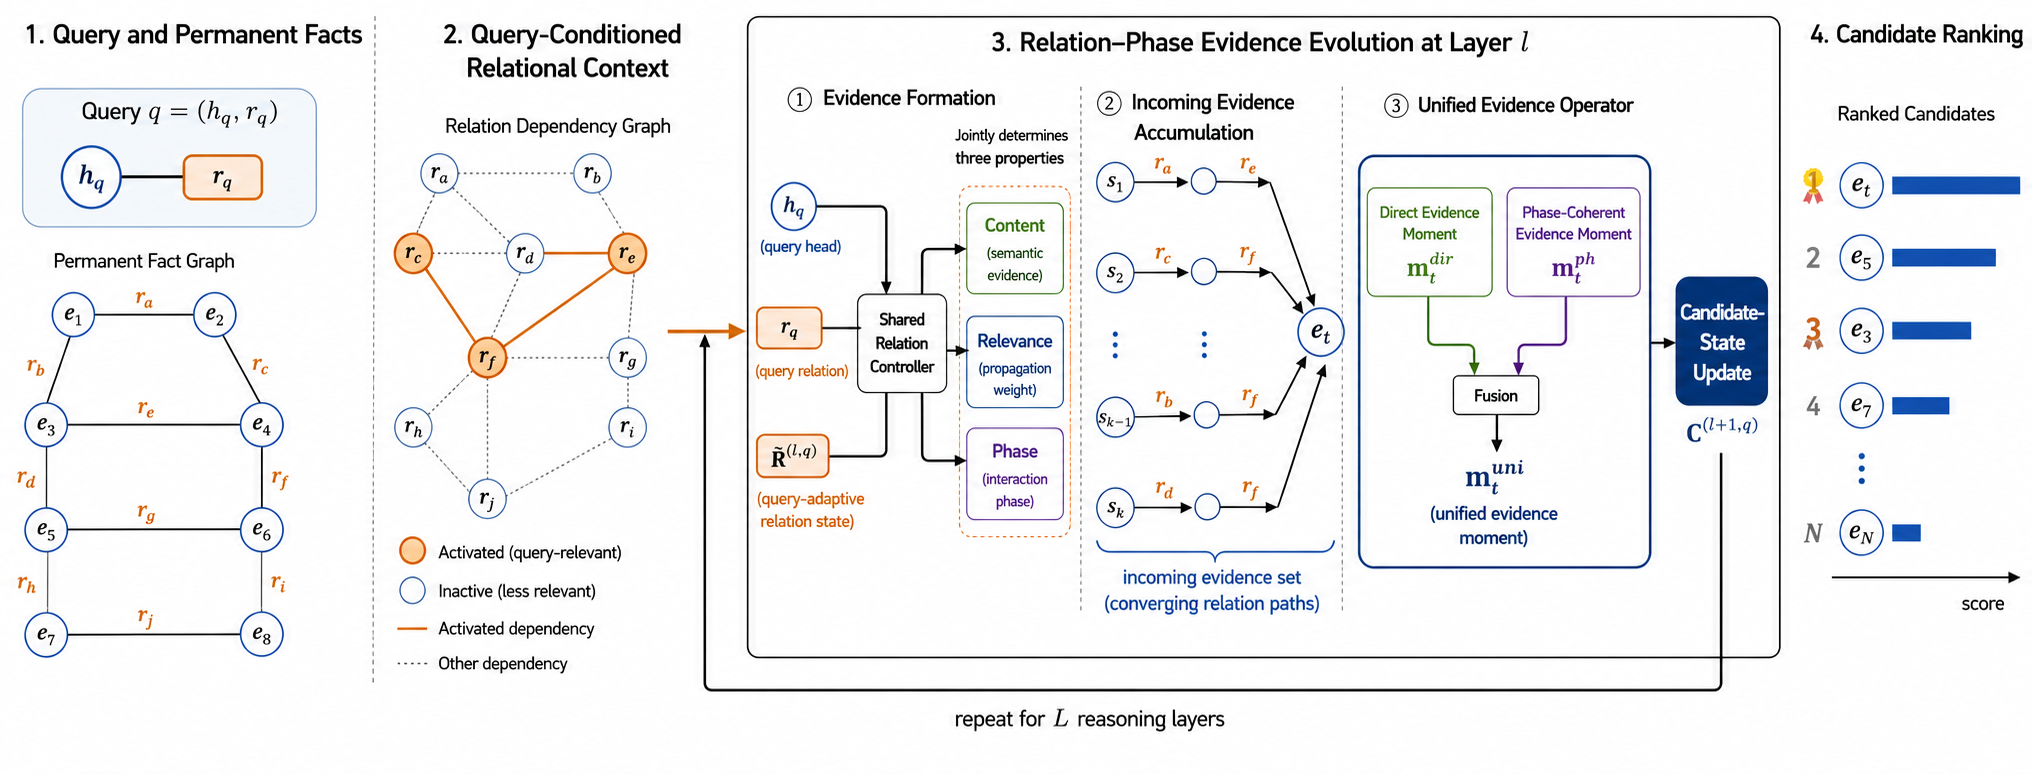
\includegraphics[width=\textwidth]{figs/rpcd-gnn-framework.png}
  \caption{Overview of RPCD-GNN. A query activates reusable relation dependencies to propagate a shared relational controller, which jointly conditions evidence content, admission strength, and interaction phase. Direct and phase-coherent evidence moments are then integrated within each recurrent reasoning layer before candidate ranking.}
  \label{fig:framework}
\end{figure*}

\subsection{Query-Conditioned Relational Context Propagation}\label{subsec:relation-codiffusion}

To make edge direction explicit, every relation $r\in\mathcal{R}$ is paired with an inverse type $r^{-1}$, and an identity relation $r_{\mathrm{id}}$ is introduced for self-propagation. The effective relation vocabulary is therefore $\mathcal{R}'=\mathcal{R}\cup\mathcal{R}^{-1}\cup\{r_{\mathrm{id}}\}$. RPCD-GNN constructs a relation dependency graph $\mathcal{G}_{r}=(\mathcal{R}',\mathcal{E}_{r})$ from recurring local relation co-occurrence patterns in a fixed fact graph. The graph encodes reusable structural associations among relations and is shared across queries, whereas its activations are dynamically conditioned on the query relation at each reasoning layer.

Let $\mathcal{A}_e$ denote the multiset of direction-aware relation incidences at entity $e$ in this fixed graph, where inverse relation types distinguish incoming from outgoing incidences and $n_e(r)$ records the multiplicity of relation $r$. Relation associations are counted between relation types sharing an anchor entity, considering only anchors that contain more than one relation incidence:
\begin{equation}
\begin{aligned}
C_{ij}
&=
\sum_{\substack{e\in\mathcal{E}\\|\mathcal{A}_e|>1}}
n_e(r_i)n_e(r_j),\\
\bar{\pi}_{ij}
&=
\begin{cases}
\dfrac{C_{ij}}{\sum_k C_{ik}},
& \sum_k C_{ik}>0,\\[5pt]
0,
& \text{otherwise}.
\end{cases}
\end{aligned}
\label{eq:relation-structural-prior}
\end{equation}
The normalized associations are filtered by a minimum-weight threshold $\delta_r$, after which source-wise Top-$K_r$ sparsification retains the most informative structural neighbors:
\begin{equation}
\mathcal{S}_{i}
=
\operatorname{TopK}_{K_r}
\left(
\left\{
j\mid j\neq i,\ \bar{\pi}_{ij}\geq\delta_r
\right\};
\bar{\pi}_{ij}
\right).
\label{eq:relation-neighborhood}
\end{equation}
A self-dependency is then added to every retained neighborhood, so $\mathcal{E}_{r}$ contains the selected pairs $(r_i,r_j)$ with $j\in\mathcal{S}_{i}$ together with $(r_i,r_i)$ for each $r_i\in\mathcal{R}'$. The corresponding edge weight is
\begin{equation}
\omega_{ij}
=
\begin{cases}
1,
& i=j,\\
\bar{\pi}_{ij},
& j\in\mathcal{S}_{i},\ i\neq j.
\end{cases}
\label{eq:relation-edge-weight}
\end{equation}
Here, $\bar{\pi}_{ij}$ is a normalized structural association rather than a deterministic logical transition probability: it reflects how frequently $r_i$ and $r_j$ participate in recurring direction-aware local association patterns, but it does not imply that one relation logically entails the other. Directionality is represented in $\mathcal{R}'$ by treating inverse relations as distinct relation types; it is therefore part of the relation vocabulary rather than a separate reasoning branch. We use $\mathcal{N}_{r}(i)$ to denote the retained neighbors of $r_i$ in $\mathcal{G}_{r}$.

We use $\operatorname{ReLU}(\cdot)$ in relation scoring and in the hidden encoders for evidence content, admission, and phase assignment. The symbol $\phi(\cdot)$ denotes the dataset-specific post-aggregation activation used in relation-state and candidate-state updates. We use $\operatorname{sigmoid}(\cdot)$ for evidence admission, $\tanh(\cdot)$ to bound the interaction phase, and $\epsilon>0$ for numerical stability. At entity reasoning layer $l$, query-conditioned relation propagation starts from the layer-specific base relation representations, i.e., $\mathbf{r}_{i}^{(l,0,q)}=\mathbf{r}_{i}^{(l)}$. For inner step $s=1,\ldots,J$ and relation edge $(r_i,r_j)\in\mathcal{E}_{r}$, the query-relation-conditioned activation is
\begin{equation}
\begin{split}
a_{ij}^{(l,s,q)}
={}&
\mathbf{w}_{r}^{\top}\operatorname{ReLU}\bigl(
W_{s}^{r}\mathbf{r}_{i}^{(l,s-1,q)}
+W_{d}^{r}\mathbf{r}_{j}^{(l,s-1,q)}\\
&\quad+W_{q}^{r}\mathbf{r}_{q}^{(l)}
+\mathbf{u}_{\omega}\log(\omega_{ij}+\epsilon)
\bigr).
\end{split}
\label{eq:query-relation-score}
\end{equation}
The activations are normalized over the retained source-wise neighborhood:
\begin{equation}
\alpha_{ij}^{(l,s,q)}
=
\frac{
\exp\left(a_{ij}^{(l,s,q)}/\tau_r\right)
}{
\sum_{k\in\mathcal{N}_{r}(i)}
\exp\left(a_{ik}^{(l,s,q)}/\tau_r\right)
}.
\label{eq:query-relation-activation}
\end{equation}
The relation state is propagated while retaining the base semantics:
\begin{equation}
\mathbf{r}_{i}^{(l,s,q)}
=
\beta\mathbf{r}_{i}^{(l)}
+
(1-\beta)
\phi\left(
\sum_{j\in\mathcal{N}_{r}(i)}
\alpha_{ij}^{(l,s,q)}
W_{m}^{r}\mathbf{r}_{j}^{(l,s-1,q)}
\right).
\label{eq:relation-state-update}
\end{equation}
After $J$ inner steps, the query-conditioned state is fused with the base relation representation:
\begin{equation}
\tilde{\mathbf{r}}_{i}^{(l,q)}
=
(1-\lambda)\mathbf{r}_{i}^{(l)}
+
\lambda\mathbf{r}_{i}^{(l,J,q)}.
\label{eq:fused-relational-context}
\end{equation}
Here, $\beta$ preserves the base relation semantics throughout inner propagation, while $\lambda$ controls how strongly the resulting query-conditioned context adapts the base relation state.
Thus, the fixed graph contributes a reusable structural prior, whereas its activation is recomputed for every query relation and reasoning layer. The resulting relational context provides a shared conditioning signal for evidence content, admission, and phase in the subsequent entity-level evolution. The relation graph is local in construction but global in use: it is distilled from reusable local relation patterns, while its query-relation-conditioned activations regulate evidence evolution throughout multi-hop reasoning.

\begin{figure*}[t]
  \centering
  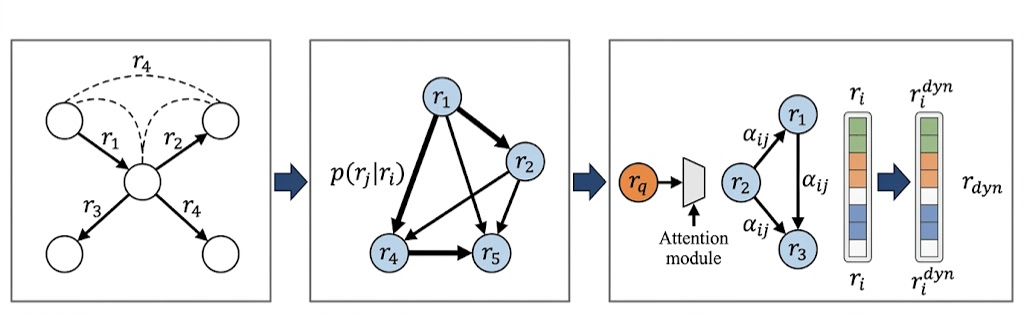
\includegraphics[width=\textwidth]{figs/relation-codiffusion.png}
  \caption{Construction and query-specific activation of the relational context. Direction-aware incidences extracted from the fixed fact graph define normalized structural associations, which are sparsified through source-wise Top-$K_r$ pruning and selectively activated by the query relation at each reasoning layer.}
  \label{fig:relation-codiffusion}
\end{figure*}

\subsection{Relation--Phase Evidence Formation}\label{subsec:entity-diffusion}

Starting from $\mathcal{V}^{(0)}=\{h_q\}$, RPCD-GNN expands the outgoing edges of the layer-wise retained entity set $\mathcal{V}^{(l-1)}$ over $\mathcal{T}_{g}$. The reached entities constitute a provisional set $\overline{\mathcal{V}}^{(l)}$, and those first reached at layer $l$ form the candidate set $\mathcal{C}^{(l)}$. For a provisional target $v$, let $\mathcal{E}_{v}^{(l)}$ denote its incoming expanded edges. The semantic content carried by an edge $(u,r,v)$ is
\begin{equation}
\mathbf{m}_{u,r,v}^{(l)}
=
\operatorname{ReLU}\left(
W_{c}^{m}
\left(
\mathbf{h}_{u}^{(l-1)}
+
\tilde{\mathbf{r}}_{r}^{(l)}
\right)
-
W_{q}^{m}
\left(
\mathbf{h}_{u}^{(l-1)}
+
\mathbf{r}_{q}^{(l)}
\right)
\right).
\label{eq:semantic-evidence-message}
\end{equation}
This contrastive composition measures the compatibility gap between the propagation relation and the query relation in the current source state. Its admission coefficient is
\begin{equation}
\gamma_{u,r,v}^{(l)}
=
\operatorname{sigmoid}\left(
\mathbf{w}_{e}^{\top}
\operatorname{ReLU}\left(
W_{h}^{e}\mathbf{h}_{u}^{(l-1)}
+
W_{r}^{e}\tilde{\mathbf{r}}_{r}^{(l)}
+
W_{q}^{e}\mathbf{r}_{q}^{(l)}
\right)
\right).
\label{eq:evidence-admission-gate}
\end{equation}
The admitted evidence is then
\begin{equation}
\mathbf{x}_{u,r,v}^{(l)}
=
\gamma_{u,r,v}^{(l)}
\mathbf{m}_{u,r,v}^{(l)}.
\label{eq:weighted-relation-evidence}
\end{equation}
Here, $\gamma_{u,r,v}^{(l)}$ controls how much semantic content is admitted into subsequent evidence interaction. Since $\mathbf{m}_{u,r,v}^{(l)}$ is produced by ReLU and $\gamma_{u,r,v}^{(l)}\in(0,1)$, the admitted evidence $\mathbf{x}_{u,r,v}^{(l)}$ is element-wise nonnegative.

To make the interaction among concurrently arriving items explicitly learnable, the same source state, relational context, and query relation parameterize an evidence phase:
\begin{equation}
\begin{split}
\theta_{u,r}^{(l)}
={}&
\pi\tanh\left(
\frac{
\mathbf{w}_{p}^{\top}
\operatorname{ReLU}\left(
W_{p}\left[
\mathbf{h}_{u}^{(l-1)};
\tilde{\mathbf{r}}_{r}^{(l)};
\mathbf{r}_{q}^{(l)}
\right]
\right)
}{
\tau_p
}
\right).
\end{split}
\label{eq:evidence-phase}
\end{equation}
The resulting complex-domain evidence item is
\begin{equation}
\mathbf{z}_{u,r,v}^{(l)}
=
\mathbf{x}_{u,r,v}^{(l)}
\exp\left(
\mathrm{i}\theta_{u,r}^{(l)}
\right).
\label{eq:complex-relation-phase-evidence}
\end{equation}
Here, $\theta_{u,r}^{(l)}\in(-\pi,\pi)$.
Equations~\eqref{eq:weighted-relation-evidence} and~\eqref{eq:complex-relation-phase-evidence} show that magnitude and phase are not produced by unrelated components. Both are query-relation-conditioned views of a single evidence item: $\mathbf{x}$ captures its admitted content, while $\theta$ specifies how that content interacts with other evidence reaching the same candidate.

\subsection{Interaction-Aware Evidence Evolution}\label{subsec:phase-interference}

\subsubsection{Direct and Phase-Coherent Evidence Moments}

Let $\mathcal{X}_{v}^{(l)}$ collect the admitted evidence and phases carried by all edges in $\mathcal{E}_{v}^{(l)}$. The direct moment retains the accumulated real-valued evidence mass:
\begin{equation}
\boldsymbol{\mu}_{v}^{(l)}
=
\sum_{(u,r,v)\in\mathcal{E}_{v}^{(l)}}
\mathbf{x}_{u,r,v}^{(l)}.
\label{eq:direct-evidence-moment}
\end{equation}
The phase-coherent moment and its element-wise amplitude are
\begin{equation}
\begin{aligned}
\boldsymbol{\kappa}_{v}^{(l)}
&=
\sum_{(u,r,v)\in\mathcal{E}_{v}^{(l)}}
\mathbf{z}_{u,r,v}^{(l)}
=
\mathbf{M}_{v}^{re,(l)}
+
\mathrm{i}\mathbf{M}_{v}^{im,(l)},\\
\boldsymbol{\rho}_{v}^{(l)}
&=
\left|
\boldsymbol{\kappa}_{v}^{(l)}
\right|
=
\sqrt{
\left(\mathbf{M}_{v}^{re,(l)}\right)^2
+
\left(\mathbf{M}_{v}^{im,(l)}\right)^2
+
\epsilon
}.
\end{aligned}
\label{eq:coherent-evidence-moment}
\end{equation}
All squared, square-root, and absolute-value operations in Eq.~\eqref{eq:coherent-evidence-moment} are applied element-wise.

The mathematical role of phase becomes clear by considering dimension $d$ of the coherent moment:
\begin{equation}
\left|
\kappa_{v,d}^{(l)}
\right|^2
=
\sum_i x_{i,d}^{2}
+
2\sum_{i<j}
x_{i,d}x_{j,d}
\cos\left(\theta_i-\theta_j\right).
\label{eq:phase-interaction-necessity}
\end{equation}
The cross terms depend on relative phase. Aligned evidence is reinforced, oppositely phased evidence is attenuated, and intermediate phase differences yield graded interactions. A conventional sum only preserves the first-order total $\sum_i x_{i,d}$ and cannot directly parameterize these pairwise compatibility terms. Phase is therefore used as a compact interaction coordinate, not as a metaphorical complex-valued decoration.

The two moments are integrated by one complex-domain evidence evolution operator:
\begin{equation}
\begin{split}
\mathcal{U}_{\mathrm{RPE}}
\left(\mathcal{X}_{v}^{(l)}\right)
=\;&
\phi\left(
W_{\mu}\boldsymbol{\mu}_{v}^{(l)}
\right)\\
&+
\eta
\phi\left(
W_{re}\operatorname{Re}
\boldsymbol{\kappa}_{v}^{(l)}
+
W_{im}\operatorname{Im}
\boldsymbol{\kappa}_{v}^{(l)}
+
W_{\rho}\boldsymbol{\rho}_{v}^{(l)}
\right).
\end{split}
\label{eq:unified-relation-phase-operator}
\end{equation}
Both moments are computed from the same relation-conditioned incoming evidence set and jointly parameterize a single candidate-state update. The direct moment preserves accumulated evidence mass, whereas the coherent moment retains phase-dependent interaction structure. Their additive projections therefore represent complementary statistics within one complex-domain evidence evolution operator.

\subsubsection{Bounded Entity Retention and Recurrent State Update}

Before recurrent evolution, RPCD-GNN limits the number of newly retained entities to prevent exponential growth of the reasoning set. For each provisional entity $v$, the unified operator output is used as its provisional state $\widehat{\mathbf{h}}_{v}^{(l)}=\mathcal{U}_{\mathrm{RPE}}(\mathcal{X}_{v}^{(l)})$. A candidate is scored by
\begin{equation}
s_{v}^{(l)}
=
\mathbf{w}_{s}^{\top}
\widehat{\mathbf{h}}_{v}^{(l)}.
\label{eq:candidate-selection-score}
\end{equation}
The layer-wise retained entity set is updated by preserving previously retained entities and adding the $K_l$ highest-scoring new candidates:
\begin{equation}
\mathcal{V}^{(l)}
=
\mathcal{V}^{(l-1)}
\cup
\operatorname{TopK}_{K_l}
\left(
\mathcal{C}^{(l)};
\widetilde{\mathbf{s}}^{(l)}
\right).
\label{eq:topk-frontier-update}
\end{equation}
Finally, evidence is accumulated recurrently over reasoning layers:
\begin{equation}
\mathbf{h}_{v}^{(l)}
=
\operatorname{GRU}\left(
\widehat{\mathbf{h}}_{v}^{(l)},
\mathbf{h}_{v}^{(l-1)}
\right),
\quad
v\in\mathcal{V}^{(l)}.
\label{eq:recurrent-entity-update}
\end{equation}
Here, $\widetilde{\mathbf{s}}^{(l)}$ denotes the Gumbel--Softmax-relaxed candidate scores with temperature $\tau_s$ during training and the deterministic scores during inference. Hard Top-$K_l$ retention uses a straight-through estimator in training so that the selection scores remain differentiable. Thus, $\mathcal{V}^{(l)}$ is a cumulative layer-wise retained entity set: it contains the previously retained entities together with the most informative newly reached candidates and supplies the source entities expanded at layer $l+1$.

For a newly retained entity, the previous state is initialized to zero. The updated state becomes the source evidence state at layer $l+1$, closing the recursive evolution from relation structure to local interaction, bounded entity retention, and multi-hop candidate semantics.

\subsection{Answer Prediction and Model Optimization}\label{subsec:model-training}

Algorithm~\ref{alg:rpcd-forward} summarizes the query-level forward process. The shared relation dependency structure is activated by the query relation at every reasoning layer.

\begin{algorithm}[t]
\caption{Query-conditioned relation propagation and complex-domain evidence evolution in RPCD-GNN}
\label{alg:rpcd-forward}
\begin{algorithmic}[1]
\Require Reasoning graph $\mathcal{T}_{g}$, relation graph $\mathcal{G}_{r}$, query $(h_q,r_q,?)$, layers $L$, relation steps $J$, retention budgets $\{K_l\}_{l=1}^{L}$
\Ensure Scores over $\mathcal{E}$
\State Initialize $\mathcal{V}^{(0)}=\{h_q\}$ and its zero state
\For{$l=1$ to $L$}
    \State Initialize $\mathbf{r}_{i}^{(l,0,q)}=\mathbf{r}_{i}^{(l)}$ and propagate $\widetilde{\mathbf{R}}^{(l,q)}$ for $J$ steps
    \State Expand $\mathcal{E}^{(l)}$ and obtain $\overline{\mathcal{V}}^{(l)}$ and $\mathcal{C}^{(l)}$
    \For{each $(u,r,v)\in\mathcal{E}^{(l)}$}
        \State Form admitted evidence $\mathbf{x}_{u,r,v}^{(l)}$
        \State Assign $\theta_{u,r}^{(l)}$ and form $\mathbf{z}_{u,r,v}^{(l)}$
    \EndFor
    \For{each $v\in\overline{\mathcal{V}}^{(l)}$}
        \State Compute $\boldsymbol{\mu}_{v}^{(l)}$, $\boldsymbol{\kappa}_{v}^{(l)}$, and $\boldsymbol{\rho}_{v}^{(l)}$
        \State Form provisional state $\widehat{\mathbf{h}}_{v}^{(l)}$
    \EndFor
    \State Score $\mathcal{C}^{(l)}$ and update the retained entity set by Eq.~\eqref{eq:topk-frontier-update}
    \For{each $v\in\mathcal{V}^{(l)}$}
        \State Evolve retained state $\mathbf{h}_{v}^{(l)}$ by Eq.~\eqref{eq:recurrent-entity-update}
    \EndFor
\EndFor
\State Project reached states and map them to the global candidate space
\State \Return $\{score(h_q,r_q,e)\mid e\in\mathcal{E}\}$
\end{algorithmic}
\end{algorithm}

After $L$ reasoning layers, the evolved candidate representations are projected and assembled into a global score vector over the entity vocabulary for answer ranking. For each candidate entity $e$, the score is computed as
\begin{equation}
score(h_q,r_q,e)
=
\mathbf{w}_{o}^{\top}
\overline{\mathbf{h}}_{e}^{(L)}.
\label{eq:global-candidate-score}
\end{equation}
The resulting score vector is used to optimize global candidate ranking. For a training query $(h_q,r_q,t)$, the loss is
\begin{equation}
\mathcal{L}
=
-
\log
\frac{
\exp\left(score(h_q,r_q,t)\right)
}{
\sum_{e\in\mathcal{E}}
\exp\left(score(h_q,r_q,e)\right)
}.
\label{eq:training-objective}
\end{equation}
At evaluation time, all entities are ranked by these scores under the filtered protocol.

\subsection{Computational Complexity}\label{subsec:computational-complexity}

Let $B$ be the query batch size, $d$ the hidden dimension, $a$ the attention dimension, $M_R$ the number of edges in the sparse relation dependency graph, and $J$ the number of relation-propagation steps within each reasoning layer. Let $M_l$ and $N_l$ denote the numbers of expanded entity edges and reached candidate nodes at layer $l$, respectively, accumulated over the batch. The per-batch online time complexity of RPCD-GNN is
\begin{equation}
\begin{split}
\mathcal{O}\!\Bigg(
\sum_{l=1}^{L}
\Biggl[
{}&BJM_R(d^2+da)
+M_l(d^2+da)
\\
{}&+N_ld^2
+B|\mathcal{E}|\log K_l
\Biggr]
\\
{}&+B|\mathcal{E}|
\Bigg).
\end{split}
\label{eq:computational-complexity}
\end{equation}
The four terms inside the summation correspond to query-relation-conditioned relation propagation, entity-edge evidence formation, phase-aware aggregation with recurrent state updates, and bounded entity retention, respectively. The last term accounts for mapping the reached states to the global score buffer and normalizing scores during optimization. The dense retention term reflects the current batched implementation, which performs Top-$K_l$ selection over an entity-wise score buffer even though message propagation is restricted to dynamically reached candidates. Since each source relation retains at most $K_r$ structural neighbors together with one self-dependency, the sparse relation graph satisfies $M_R\leq|\mathcal{R}'|(K_r+1)$. Consequently, the online relation-context overhead is bounded by $\mathcal{O}(BLJ|\mathcal{R}'|(K_r+1)(d^2+da))$, which depends on the relation vocabulary rather than the number of entities once the relation graph has been precomputed. Before training, the unpruned relation dependency graph is constructed once in $\mathcal{O}(\sum_{e\in\mathcal{E}}c_e^2)$ time, where $c_e=|\mathcal{A}_e|$ is the number of direction-aware relation incidences at entity $e$, and is subsequently sparsified by relation-wise Top-$K_r$ pruning. Beyond the entity-state tensors required by progressive propagation, the principal additional memory terms are $\mathcal{O}(B|\mathcal{R}'|d+M_R)$ for query-relation-conditioned relation states and the sparse relation graph, where $|\mathcal{R}'|=2|\mathcal{R}|+1$ includes original, inverse, and identity relations.

\section{Experiments}\label{sec:experiments}

\subsection{Datasets}\label{subsec:datasets}

We evaluate RPCD-GNN on five transductive knowledge graph reasoning datasets, including Family, UMLS, WN18RR, NELL-995, and FB15k-237. These datasets cover different graph scales, relation densities, and reasoning patterns, allowing us to examine query-conditioned relation propagation and complex-domain evidence evolution in both small-scale logical reasoning and large-scale knowledge graph scenarios.

Family is a relational reasoning dataset derived from kinship relations, where the target is to infer implicit family relations from observed relational facts \citep{Kok2007Statistical,Sadeghian2019DRUM}. UMLS is a biomedical relational dataset constructed from the Unified Medical Language System and is commonly used to evaluate multi-relational reasoning over medical concepts \citep{Bodenreider2004UMLS,Sadeghian2019DRUM}. WN18RR is a leakage-reduced subset of WordNet that removes inverse-relation shortcuts from WN18 and therefore requires models to exploit more meaningful relational evidence \citep{Dettmers2018ConvE}. FB15k-237 is derived from Freebase by removing near-duplicate and inverse relations, making it a challenging benchmark for relation prediction \citep{Toutanova2015Observed,Dettmers2018ConvE}. NELL-995 is a large-scale knowledge graph reasoning dataset constructed from the Never-Ending Language Learning project and contains more entities and sparse relational patterns \citep{Xiong2017DeepPath}.

The released benchmark files contain a permanent fact set $\mathcal{T}_{f}$, a training set $\mathcal{T}_{tr}$, a validation set $\mathcal{T}_{va}$, and a test set $\mathcal{T}_{te}$. Their statistics are summarized in Table~\ref{tab:dataset-statistics}; the graph--query construction used at each experimental stage is detailed in Section~\ref{subsec:implementation-details}.

\begin{table*}[t]
\caption{Statistics of the transductive reasoning datasets. Relation and triple counts are reported before augmentation with inverse relations and identity self-loops.}
\label{tab:dataset-statistics}
\centering
\begin{tabular}{lrrrrrr}
\hline
Dataset & Entities & Relations & Facts & Train & Valid & Test \\
\hline
Family & 3,007 & 12 & 17,615 & 5,868 & 2,038 & 2,835 \\
UMLS & 135 & 46 & 4,006 & 1,321 & 569 & 633 \\
WN18RR & 40,943 & 11 & 65,130 & 21,705 & 3,034 & 3,134 \\
NELL-995 & 74,536 & 200 & 112,258 & 37,420 & 543 & 2,818 \\
FB15k-237 & 14,541 & 237 & 204,087 & 68,028 & 17,535 & 20,466 \\
\hline
\end{tabular}
\end{table*}

\subsection{Baselines and Evaluation Metrics}\label{subsec:baselines-metrics}

We compare RPCD-GNN with representative knowledge graph reasoning methods from complementary reasoning paradigms. The non-GNN baselines include embedding-based models ConvE \citep{Dettmers2018ConvE}, QuatE \citep{Zhang2019QuatE}, and RotatE \citep{Sun2019RotatE}; path- and rule-based reasoners MINERVA \citep{Das2018MINERVA}, DRUM \citep{Sadeghian2019DRUM}, RNNLogic \citep{Qu2021RNNLogic}, and RLogic \citep{Cheng2022RLogic}; and parameter-efficient representation models NodePiece \citep{Galkin2022NodePiece} and MorsE with RotatE as its base scoring function \citep{Chen2021MorsE}. Together, they provide comparisons from triple scoring, explicit relational composition, and parameter-efficient representation learning perspectives.

The GNN-based baselines include CompGCN \citep{Vashishth2020CompGCN}, NBFNet \citep{Zhu2021NBFNet}, RED-GNN \citep{Zhang2022REDGNN}, AdaProp \citep{Zhang2023AdaProp}, A*Net \citep{Zhu2023AStarNet}, DiffusionE \citep{Cao2024DiffusionE}, and Top-p reasoning \citep{Liu2025TopPReasoning}. CompGCN represents full-graph relational aggregation, whereas NBFNet, RED-GNN, AdaProp, A*Net, DiffusionE, and Top-p reasoning instantiate different forms of query-dependent progressive propagation. The comparison includes representative reasoning methods whose dataset splits and filtered-ranking protocols are compatible with our setting.

Following the standard filtered-ranking protocol, we evaluate both tail prediction and head prediction, where head-prediction queries are converted into tail-prediction queries using inverse relations. For each query, all entities are ranked according to their prediction scores, while other known correct answers in $\mathcal{T}_{f}\cup\mathcal{T}_{tr}\cup\mathcal{T}_{va}\cup\mathcal{T}_{te}$ are removed only when computing the rank of the target entity. We report mean reciprocal rank (MRR), Hits@1, and Hits@10, with higher values indicating better reasoning performance.

\subsection{Implementation Details}\label{subsec:implementation-details}

At each training epoch $s$, $\mathcal{T}_{f}$ and $\mathcal{T}_{tr}$ are pooled and randomly repartitioned according to the dataset-specific fact ratio $\varrho$. The retained triples form the current reasoning graph $\mathcal{T}_{g}^{(s)}$, while the remaining triples provide supervised queries $\mathcal{T}_{q}^{(s)}$. During validation and testing, $\mathcal{T}_{f}\cup\mathcal{T}_{tr}$ forms the fixed reasoning graph, and queries are drawn from $\mathcal{T}_{va}$ and $\mathcal{T}_{te}$, respectively. The relation dependency graph is constructed once from $\mathcal{T}_{f}$ and remains fixed throughout training and evaluation. For FB15k-237, direct one-hop connections associated with the current training queries are removed from $\mathcal{T}_{g}^{(s)}$ following the released backbone protocol.

RPCD-GNN is implemented in PyTorch and optimized using Adam on a single NVIDIA GPU. Inverse relations and identity self-loops are included in the entity message-passing graph, and inverse relation types are also used in the direction-aware incidences defined in Section~\ref{subsec:relation-codiffusion}. The query-conditioned activations of the fixed relation dependency graph are recomputed at every entity reasoning layer. Following the released transductive configurations of DiffusionE \citep{Cao2024DiffusionE}, we retain its dataset-specific propagation depth, retention budget, batch size, fact ratio, and optimization settings. The model is trained for at most 300 epochs with an exponentially decayed learning rate, and the checkpoint achieving the highest validation MRR is used for final evaluation. RPCD-specific parameters $K_r$, $\delta_r$, $J$, $\lambda$, $\beta$, $\eta$, $\tau_r$, and $\tau_p$ are selected according to validation MRR. Final results are reported as the mean and standard deviation over three independent runs.

% TODO(final experiments): specify the GPU model and software versions.
\begin{table*}[t]
\caption{Dataset-specific backbone and training configurations used in the experiments.}
\label{tab:implementation-settings}
\centering
\small
\setlength{\tabcolsep}{4pt}
\begin{tabular}{lrrrrrrrrl}
\toprule
Dataset & $d$ & $a$ & $L$ & $K_l$ & $\varrho$ & Batch & LR & WD & Activation \\
\midrule
Family & 48 & 5 & 8 & 100 & 0.90 & 20 & 0.0036 & 0.000017 & ReLU \\
UMLS & 64 & 5 & 5 & 100 & 0.90 & 10 & 0.0012 & 0.000140 & tanh \\
WN18RR & 64 & 5 & 8 & 1000 & 0.96 & 50 & 0.0030 & 0.000140 & identity \\
FB15k-237 & 48 & 5 & 7 & 2000 & 0.99 & 6 & 0.0009 & 0.000080 & identity \\
NELL-995 & 128 & 64 & 6 & 2000 & 0.95 & 10 & 0.0011 & 0.000089 & identity \\
\bottomrule
\end{tabular}
\end{table*}

\subsection{Results and Analysis}\label{subsec:results-analysis}

All reported results follow the transductive filtered-ranking protocol described above. RPCD-GNN checkpoints are selected exclusively according to validation MRR. Literature results are included only when the dataset partition, candidate-ranking space, and filtering protocol are compatible with our setting.

\begin{table*}[t]
\caption{Experimental results on Family and UMLS. The best and second-best results are highlighted in bold and underlined, respectively.}
\label{tab:main-results-small}
\centering
\small
\setlength{\tabcolsep}{5pt}
\begin{tabular}{llcccccc}
\hline
Type & Model
& \multicolumn{3}{c}{Family}
& \multicolumn{3}{c}{UMLS} \\
\cline{3-8}
& & MRR & H@1 & H@10 & MRR & H@1 & H@10 \\
\hline
non-GNN & ConvE & 0.912 & 0.837 & 0.982 & 0.937 & 0.922 & 0.967 \\
 & QuatE & 0.941 & 0.896 & 0.991 & 0.944 & 0.905 & 0.993 \\
 & RotatE & 0.921 & 0.866 & 0.988 & 0.925 & 0.863 & 0.993 \\
 & MINERVA & 0.885 & 0.825 & 0.961 & 0.825 & 0.728 & 0.968 \\
 & DRUM & 0.934 & 0.881 & \underline{0.996} & 0.813 & 0.674 & 0.976 \\
 & RNNLogic & 0.881 & 0.857 & 0.907 & 0.842 & 0.772 & 0.965 \\
 & NodePiece & 0.892 & 0.837 & 0.971 & 0.844 & 0.736 & 0.968 \\
 & MorsE (RotatE) & 0.938 & 0.886 & 0.994 & 0.815 & 0.679 & 0.978 \\
\hline
GNN & CompGCN & 0.933 & 0.883 & 0.991 & 0.927 & 0.867 & 0.994 \\
 & NBFNet & 0.989 & \underline{0.988} & 0.989 & 0.948 & 0.920 & \underline{0.995} \\
 & RED-GNN & \textbf{0.992} & \underline{0.988} & \textbf{0.997} & 0.964 & 0.946 & 0.990 \\
 & AdaProp & 0.988 & 0.986 & 0.990 & 0.969 & 0.956 & \underline{0.995} \\
 & DiffusionE & \underline{0.990} & \textbf{0.989} & 0.992 & \underline{0.970} & \underline{0.957} & 0.992 \\
 & RPCD-GNN & \underline{0.990} & \textbf{0.989} & 0.991 & \textbf{0.982} & \textbf{0.971} & \textbf{0.996} \\
\hline
\end{tabular}
\end{table*}

\begin{table*}[t]
\caption{Experimental results on WN18RR, FB15k-237, and NELL-995. The best and second-best results are highlighted in bold and underlined, respectively.}
\label{tab:main-results-large}
\centering
\small
\setlength{\tabcolsep}{3.5pt}
\begin{tabular}{lccccccccc}
\hline
Model
& \multicolumn{3}{c}{WN18RR}
& \multicolumn{3}{c}{FB15k-237}
& \multicolumn{3}{c}{NELL-995} \\
\cline{2-10}
& MRR & H@1 & H@10 & MRR & H@1 & H@10 & MRR & H@1 & H@10 \\
\hline
NBFNet & 0.551 & 0.497 & 0.666 & \underline{0.415} & \underline{0.321} & \textbf{0.599} & 0.525 & 0.451 & 0.639 \\
RED-GNN & 0.533 & 0.485 & 0.624 & 0.374 & 0.283 & 0.558 & 0.543 & 0.476 & 0.651 \\
AdaProp & \underline{0.562} & 0.499 & 0.671 & \textbf{0.417} & \textbf{0.331} & 0.585 & \underline{0.554} & \underline{0.493} & \underline{0.655} \\
A*Net & 0.549 & 0.495 & 0.659 & 0.411 & \underline{0.321} & \underline{0.586} & -- & -- & -- \\
DiffusionE & 0.557 & \underline{0.504} & 0.658 & 0.376 & 0.294 & 0.539 & 0.552 & 0.490 & 0.654 \\
Top-p reasoning & 0.559 & 0.498 & \underline{0.676} & -- & -- & -- & \textbf{0.559} & \textbf{0.496} & \textbf{0.662} \\
RPCD-GNN & \textbf{0.576} & \textbf{0.524} & \textbf{0.679} & -- & -- & -- & -- & -- & -- \\
\hline
\end{tabular}
\end{table*}

Table~\ref{tab:main-results-small} presents the comparison on the compact Family and UMLS reasoning benchmarks, whereas Table~\ref{tab:main-results-large} reports results on WN18RR, FB15k-237, and NELL-995. The currently available RPCD-GNN entries in both tables are retained only as preliminary single-run evidence and are not used to make final state-of-the-art or statistical claims.

After the repeated runs are completed, the analysis will first compare RPCD-GNN with representative methods from different reasoning paradigms and then discuss its performance across datasets with different graph and relational characteristics. The current highlighting reflects the values displayed in the tables and will be updated together with the absolute and relative improvements after all results have been verified under compatible protocols. The effects of query-conditioned relational context and phase-coherent evidence aggregation are examined separately in the subsequent ablation and mechanism analyses.

The dataset-level discussion will distinguish saturated benchmarks, such as Family, from datasets with richer relation vocabularies or larger reasoning spaces. Explanations based on relation complexity, multi-hop evidence interaction, or graph scale will be stated only when supported jointly by the final main results, ablations, and mechanism analyses.

\subsection{Ablation Study}\label{subsec:ablation-study}

To assess how query-conditioned relational context and phase-coherent evidence aggregation affect reasoning performance, we construct two controlled variants of RPCD-GNN. RPCD-GNN w/o relational context disables query-conditioned relation propagation and uses the base relation representations during evidence formation. RPCD-GNN w/o phase-coherent evidence removes the coherent evidence moment and retains direct evidence accumulation for candidate-state evolution. All other configurations remain unchanged.

\begin{table*}[t]
\caption{Ablation results of RPCD-GNN on WN18RR, FB15k-237, and NELL-995. The displayed full-model values are preliminary single-run results; ``--'' denotes a pending controlled run.}
\label{tab:ablation-modules}
\centering
\small
\setlength{\tabcolsep}{4pt}
\begin{tabular}{lrrrrrr}
\hline
Variant
& \multicolumn{2}{c}{WN18RR}
& \multicolumn{2}{c}{FB15k-237}
& \multicolumn{2}{c}{NELL-995} \\
\cline{2-7}
& MRR & H@10 & MRR & H@10 & MRR & H@10 \\
\hline
RPCD-GNN w/o relational context & -- & -- & -- & -- & -- & -- \\
RPCD-GNN w/o phase-coherent evidence & -- & -- & -- & -- & -- & -- \\
RPCD-GNN & 0.576 & 0.679 & -- & -- & -- & -- \\
\hline
\end{tabular}
\end{table*}

The comparison evaluates how query-conditioned relational context and phase-coherent evidence aggregation affect reasoning performance under the same experimental configuration. Conclusions about their effects will be drawn only from the completed controlled runs. Entries marked ``--'' are intentionally left pending; no ablation result is inferred from the currently available full-model score.

\subsection{Relation Dependency Analysis}\label{subsec:relation-dependency-analysis}

We analyze the sparse relation dependency graphs constructed on the five datasets. The reported statistics characterize the effective relation vocabulary, the number of candidate dependencies before pruning, and the relational structure retained after relation-wise Top-$K_r$ pruning. We report the number of effective relation types, candidate non-self dependencies, retained non-self dependencies, graph density, average non-self degree, and relation coverage. Identity self-dependencies are excluded from the density, degree, and coverage statistics.

\begin{table*}[t]
\caption{Statistics of the sparse relation dependency graphs. ``--'' denotes a pending statistic.}
\label{tab:relation-dependency-statistics}
\centering
\small
\setlength{\tabcolsep}{4pt}
\begin{tabular}{lrrrrrr}
\hline
Dataset & $|\mathcal{R}'|$ & Candidate deps. & Retained deps. & Density & Avg. degree & Coverage \\
\hline
Family & -- & -- & -- & -- & -- & -- \\
UMLS & -- & -- & -- & -- & -- & -- \\
WN18RR & -- & -- & -- & -- & -- & -- \\
FB15k-237 & -- & -- & -- & -- & -- & -- \\
NELL-995 & -- & -- & -- & -- & -- & -- \\
\hline
\end{tabular}
\end{table*}

Candidate dependencies count non-self relation pairs before pruning, whereas retained dependencies count those preserved after Top-$K_r$ pruning. Density is measured over all possible directed non-self relation pairs, average degree is the mean retained non-self out-degree, and coverage is the proportion of relation types with at least one retained non-self neighbor. These statistics will be used to examine how much recurring relational structure is preserved by the sparse graph without making an empirical efficiency claim.

\subsection{Parameter Sensitivity Analysis}\label{subsec:parameter-sensitivity}

The sensitivity study varies four key hyperparameters one at a time on WN18RR and FB15k-237 while holding the remaining validation-selected configuration fixed, as organized in Fig.~\ref{fig:parameter-sensitivity}. The relation adaptation weight $\lambda$ (\texttt{rel\_diff\_weight}) controls the contribution of query-adaptive relation semantics, and the relation-neighbor budget $K_r$ (\texttt{rel\_line\_topk}) controls the sparsity of the structural relation prior. The coherent-moment weight $\eta$ (\texttt{phase\_weight}) controls the contribution of phase-coherent evidence to the candidate-state update, while the phase temperature $\tau_p$ (\texttt{phase\_tau}) controls the dispersion of interaction phases. The search grids are $\lambda\in\{0.1,0.3,0.5,0.7,1.0\}$, $K_r\in\{5,10,20,\mathrm{All}\}$, $\eta\in\{0.1,0.2,0.3,0.5,0.7\}$, and $\tau_p\in\{0.5,1.0,2.0\}$. Validation MRR is reported for every sweep, and the test set is not used to choose the operating point.

\begin{figure*}[t]
  \centering
  % TODO(figure polish): The phase contribution weight in the artwork must be
  % denoted by \eta rather than \beta; \beta is reserved for relation residuals.
  % TODO(final experiments): Replace the data-free template with validation-MRR
  % curves generated from the controlled parameter sweeps.
  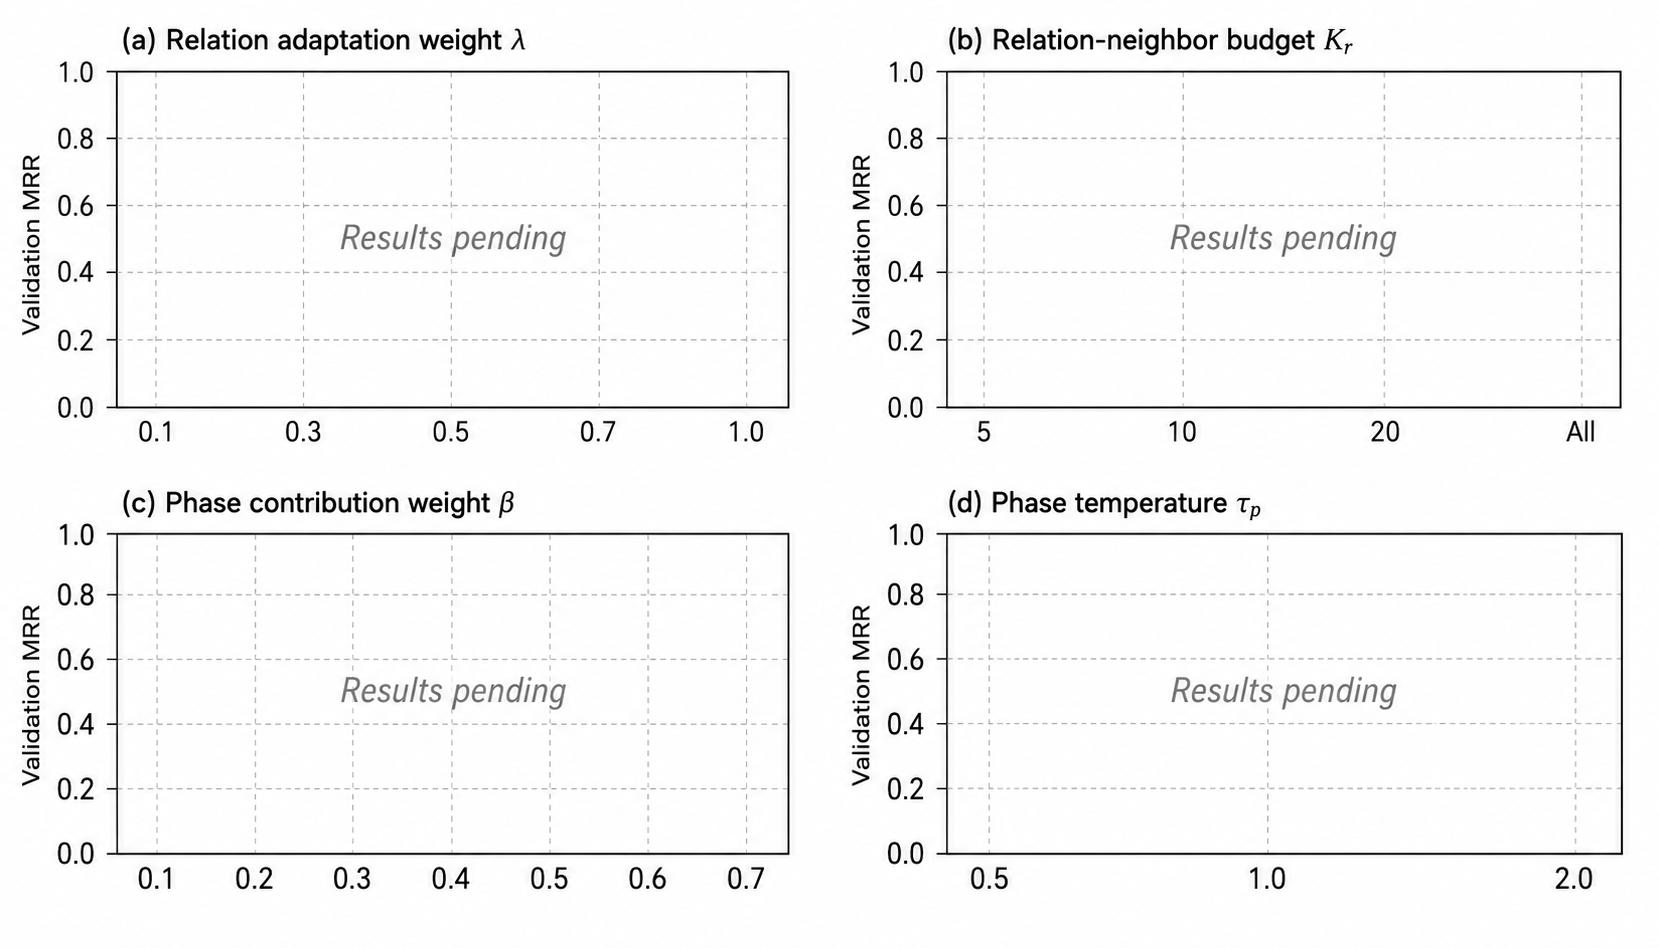
\includegraphics[width=0.95\textwidth]{figs/parameter-sensitivity.png}
  \caption{Sensitivity of RPCD-GNN to the relation adaptation weight $\lambda$, relation-neighbor budget $K_r$, coherent-moment weight $\eta$, and phase temperature $\tau_p$ on WN18RR and FB15k-237.}
  \label{fig:parameter-sensitivity}
\end{figure*}

The analysis examines how the scope of relational context and the contribution of phase-coherent evidence affect validation performance without assuming a preferred trend before the controlled sweeps are completed. The final discussion will distinguish broad stable regions from isolated best points and will attribute a trend to the corresponding design only when it is consistent across the reported datasets.

\subsection{Phase Coherence Analysis}\label{subsec:phase-coherence-analysis}

To examine how the learned interaction phases organize convergent evidence, we compare the complex-evidence coherence scores of correct targets with those of high-ranking incorrect candidates on WN18RR and FB15k-237. For each test query, the hard negative is defined as the highest-ranked incorrect candidate after filtered evaluation. Given the complex evidence vectors $\mathbf{z}_{i}^{(l)}$ arriving at candidate $v$ in layer $l$, its complex-evidence coherence score is

\[
\chi_{v}^{(l)}=
\frac{\left\|\sum_i \mathbf{z}_{i}^{(l)}\right\|_2}
{\sum_i\left\|\mathbf{z}_{i}^{(l)}\right\|_2+\epsilon}.
\]

A larger score indicates stronger directional alignment among the complex evidence vectors reaching the candidate. To avoid the trivial coherence of a single evidence item, the reported distributions include only candidates that receive at least two incoming evidence items; the corresponding sample counts will be reported with the final results.

\begin{figure*}[t]
  \centering
  % TODO(final experiments): Replace the placeholder with box or violin plots
  % computed from model-traced evidence on WN18RR and FB15k-237.
  \IfFileExists{figs/phase-coherence-analysis.png}
    {\includegraphics[width=0.95\textwidth]{figs/phase-coherence-analysis.png}}
    {\fbox{\parbox[c][55mm][c]{0.9\textwidth}{\centering
      Phase-coherence figure placeholder\\
      Upload \texttt{figs/phase-coherence-analysis.png}}}}
  \caption{Complex-evidence coherence distributions of correct targets and high-ranking incorrect candidates on WN18RR and FB15k-237.}
  \label{fig:phase-coherence-analysis}
\end{figure*}

Fig.~\ref{fig:phase-coherence-analysis} will report the final-layer distributions for correct targets and hard negatives using the same trained model and filtering protocol. The interpretation will be based on the observed distributions rather than assuming in advance that correct candidates must exhibit higher coherence.

\subsection{Case Study}\label{subsec:case-study}

We trace one successful query and one failure case on FB15k-237 to illustrate how relation-conditioned evidence affects candidate ranking. For each query, the analysis reports the dominant layer-wise evidence traces, relation sequences, evidence strengths, relative phases, contribution scores, and the change in target rank between direct-only aggregation and the complete RPCD-GNN. The queries will be selected according to a fixed rank-based criterion before their evidence traces are inspected rather than by manual preference.

\begin{figure*}[t]
  \centering
  % TODO(final experiments): Replace the illustrative traces, phases,
  % contributions, and rank placeholders with model-traced evidence.
  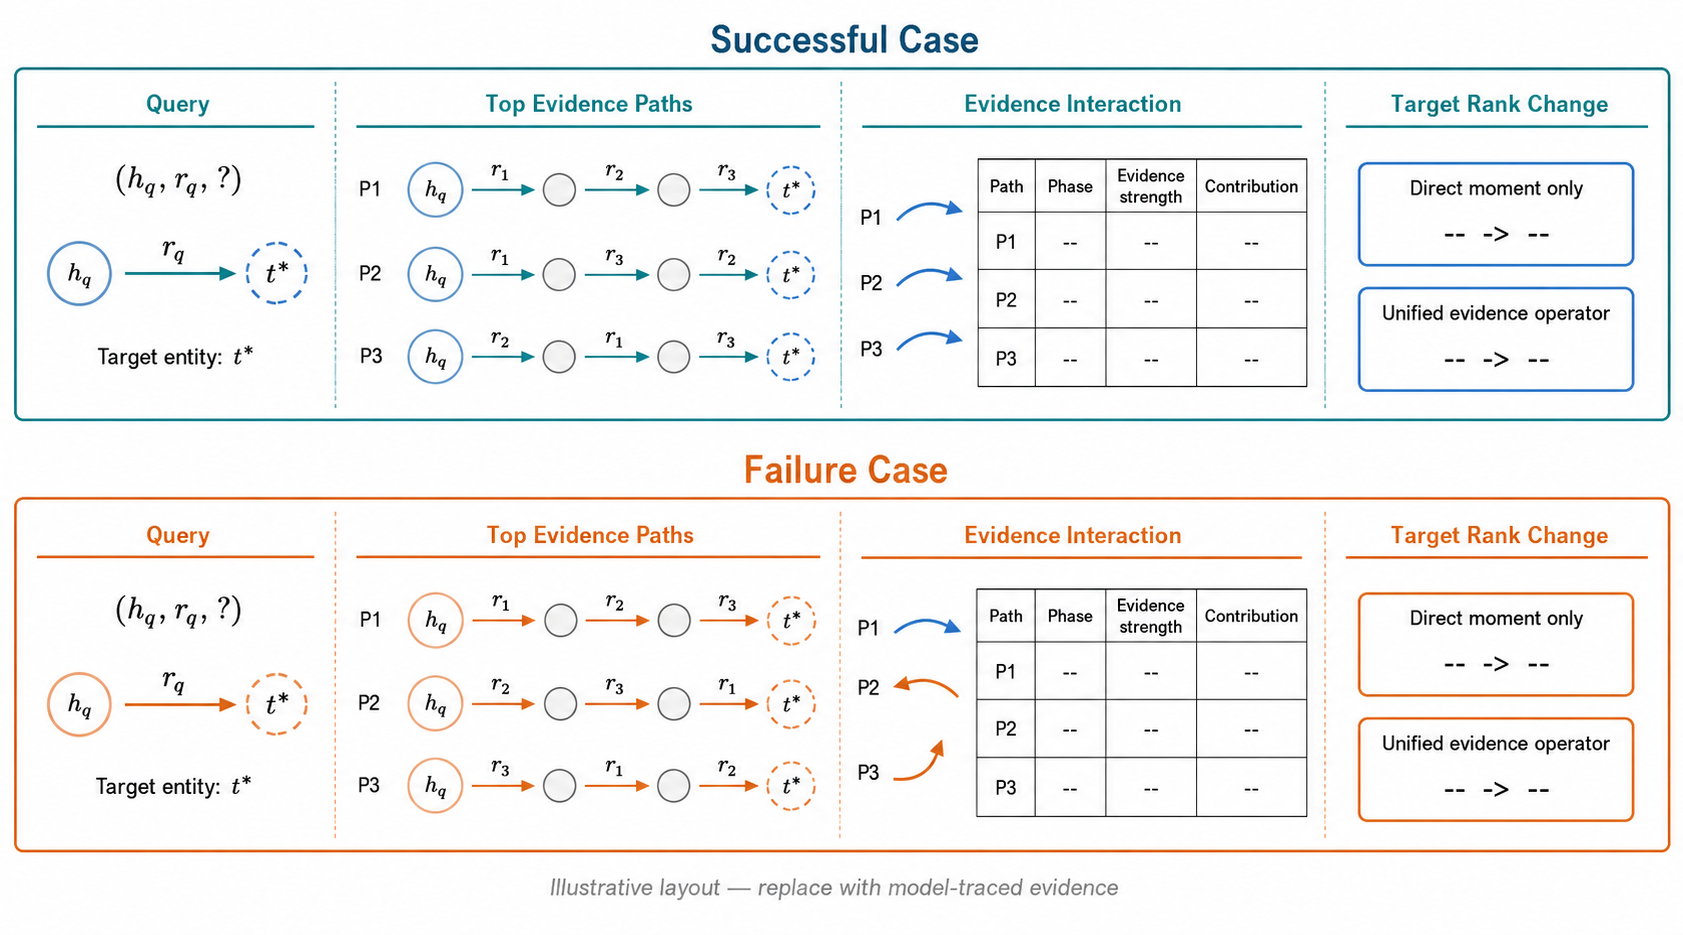
\includegraphics[width=0.95\textwidth]{figs/reasoning-path-case-study.png}
  \caption{Evidence analysis of representative successful and failure queries on FB15k-237, including dominant evidence traces, relative phases, contribution scores, and target-rank changes.}
  \label{fig:reasoning-path-case}
\end{figure*}

Fig.~\ref{fig:reasoning-path-case} will annotate the dominant evidence traces, their relation sequences, strengths, relative phases, contributions, and changes in the target rank. The successful case will examine whether phase-aligned evidence receives a stronger coherent response, while the failure case will identify situations in which weakly aligned or noisy evidence still dominates candidate prediction. This paired presentation is intended to illustrate both the capability and the limitation of the phase-coherent update rather than infer a general mechanism from a single favorable example.

\section{Conclusion}\label{sec:conclusion}

In this paper, we proposed RPCD-GNN, a query-conditioned framework that couples relation propagation with complex-domain evidence evolution for knowledge graph reasoning. RPCD-GNN addresses the separation between relation-level structural modeling and multi-path evidence interaction by organizing relational context formation, relation-conditioned evidence construction, cross-evidence interaction, and candidate-state evolution within a unified recurrent process. In this process, query-adaptive relation states jointly condition the semantic content, admission strength, and interaction phase of evidence, allowing relational dependencies to regulate how different reasoning paths contribute to candidate prediction.

Rather than treating path-wise messages as independent contributions, RPCD-GNN summarizes incoming evidence through complementary direct and phase-coherent evidence moments and uses their joint response to drive candidate-state evolution across reasoning layers. This formulation represents both the direct accumulation of relational evidence and the structured interaction among converging reasoning paths within a common complex-domain evolution mechanism.

% TODO: Add the final empirical conclusion based on the main results,
% ablation study, relation dependency analysis, and phase coherence analysis.

Future work will extend query-conditioned relation propagation to larger and dynamically evolving knowledge graphs and incorporate textual or temporal signals into complex-domain evidence evolution, enabling the framework to reason under richer and less stationary semantic contexts.

% Numbered list
% Use the style of numbering in square brackets.
% If nothing is used, default style will be taken.
%\begin{enumerate}[a)]
%\item 
%\item 
%\item 
%\end{enumerate}  

% Unnumbered list
%\begin{itemize}
%\item 
%\item 
%\item 
%\end{itemize}  

% Description list
%\begin{description}
%\item[]
%\item[] 
%\item[] 
%\end{description}  

% Figure
%\begin{figure}%[]
%  \centering
%%    \includegraphics{}
%    \caption{}\label{fig1}
%\end{figure}


%\begin{table}%[]
%\caption{}\label{tbl1}
%\begin{tabular*}{\tblwidth}{@{}LL@{}}
%\toprule
%  &  \\ % Table header row
%\midrule
% & \\
% & \\
% & \\
% & \\
%\bottomrule
%\end{tabular*}
%\end{table}

% Uncomment and use as the case may be
%\begin{theorem} 
%\end{theorem}

% Uncomment and use as the case may be
%\begin{lemma} 
%\end{lemma}

%% The Appendices part is started with the command \appendix;
%% appendix sections are then done as normal sections
%% \appendix

%\section{}\label{}

% To print the credit authorship contribution details
\printcredits

%% Loading bibliography style file
%\bibliographystyle{model1-num-names}
\bibliographystyle{cas-model2-names}

% Loading bibliography database
\bibliography{cas-refs}

% Biography
%\bio{}
% Here goes the biography details.
%\endbio

%\bio{pic1}
% Here goes the biography details.
%\endbio

\end{document}
